% (The MIT License)
%
% Copyright (c) 2023-2024 Yegor Bugayenko
%
% Permission is hereby granted, free of charge, to any person obtaining a copy
% of this software and associated documentation files (the 'Software'), to deal
% in the Software without restriction, including without limitation the rights
% to use, copy, modify, merge, publish, distribute, sublicense, and/or sell
% copies of the Software, and to permit persons to whom the Software is
% furnished to do so, subject to the following conditions:
%
% The above copyright notice and this permission notice shall be included in all
% copies or substantial portions of the Software.
%
% THE SOFTWARE IS PROVIDED 'AS IS', WITHOUT WARRANTY OF ANY KIND, EXPRESS OR
% IMPLIED, INCLUDING BUT NOT LIMITED TO THE WARRANTIES OF MERCHANTABILITY,
% FITNESS FOR A PARTICULAR PURPOSE AND NONINFRINGEMENT. IN NO EVENT SHALL THE
% AUTHORS OR COPYRIGHT HOLDERS BE LIABLE FOR ANY CLAIM, DAMAGES OR OTHER
% LIABILITY, WHETHER IN AN ACTION OF CONTRACT, TORT OR OTHERWISE, ARISING FROM,
% OUT OF OR IN CONNECTION WITH THE SOFTWARE OR THE USE OR OTHER DEALINGS IN THE
% SOFTWARE.

\documentclass{article}
\usepackage{../osbp}
\newcommand*\thetitle{Reviewing Changes}
\begin{document}

\plush{\osbpTitlePage{4}{}}

\pitch{.}

% when and how we reject PRs?
%

% Effects of personality traits on pull request acceptance
% RN Iyer, SA Yun, M Nagappan, J Hoey - IEEE Transactions on Software Engineering, 2019

% start from this:
% https://dl.acm.org/doi/pdf/10.1145/3183519.3183525

\qte
  [Michael Fagan]
  {michael-fagan.jpg}
  {The inspection is not intended to redesign, evaluate alternate design solutions, or to find solutions to errors; it is intended \ul{just} to find errors!}
  {fagan1976design}

\qte
  [Alberto Bacchelli]
  {alberto-bacchelli}
  {Our results show that, although the top motivation driving code reviews is still finding defects, the practice and the actual outcomes are \ul{less} about finding errors than expected: Defect related comments comprise a small proportion and mainly cover small logical low-level issues.}
  {bacchelli2013expectations}

\qte
  [Mateus Freira dos Santos]
  {mateus-freira-dos-santos}
  {In software projects with less than 34k lines of code, the number of developers that \ul{never contribute again} after receiving a negative comment on the first pull request is 10.97\%; this number more than doubles to 24.02\% when evaluating projects with more than 197k lines of code.}
  {mateus-freira-dos-santos.jpg}

\qte
  [Andrew Sutherland]
  {andrew-sutherland}
  {The meat of the code review dialog, no matter what the medium, is the articulation of design rationale... Engineers find code review dialogs useful for a variety of purposes, but for understanding design rationale more than any other.}
  {sutherland2009can}

\qte
  [Frank A. Ackerman]
  {frank-ackerman}
  {Regardless of the application or the language, you can expect inspections to find from seven to 20 major \ul{defects} per thousand noncomment lines of source code and to find major defects at a \ul{cost} of one to five staff-hours.}
  {ackerman1989software}

\qte
  [Caitlin Sadowski]
  {caitlin-sadowski}
  {As developers build experience working at Google, the average number of comments on their changes decreases... Developers at Google who have started within the past year typically have more than twice as many comments per change.}
  {sadowski2018modern}
\pitch{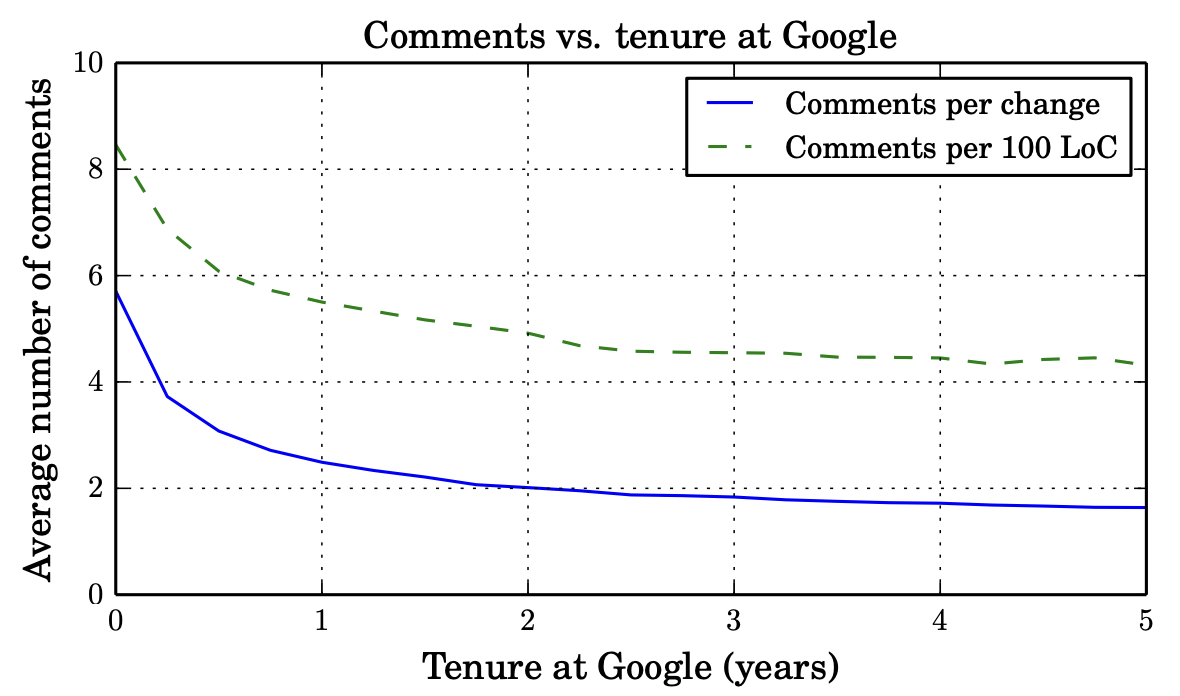
\includegraphics[width=.95\linewidth]{tenure.png}}

\qte
  {eric-raymond}
  {Good programmers know what to write. Great ones know what to rewrite (and reuse).}
  {raymond1999cathedral}

\thought[bugayenko2019blog1203]{Don't run the code in the branch}

\thought{Rely on the CI status, but not too much}

\qte
  [Mairieli Wessel]
  {mairieli-wessel}
  {Our findings also suggest that the adoption of GitHub Actions leads to more rejections of pull requests (PRs), more communication in accepted PRs and less communication in rejected PRs, fewer commits in accepted PRs and more commits in rejected PRs, and more time to accept a PR.}
  {wessel2023github}

\thought[bugayenko2015blog0209]{Make not compromises}

\thought[bugayenko2015blog0209]{Have no fear}

\thought[bugayenko2015blog0622]{Reject it, if it doesn't reproduce a bug}

\thought[bugayenko2015blog0622]{Reject it, if it lowers code coverage}

\end{document}
